\section{连续映射}
\label{sec:metric-continuous-maps}

前面几节研究一个空间内部的点和集合。现在固定两个度量空间$(X,d_X)$、$(Y,d_Y)$和一个映射$f:D\to Y$，其中$D\subseteq X$配备子空间度量，问输入的小误差能否保证输出的小误差。本节先定义函数极限与连续性，再按“容差是否随位置变化”“输出误差能否被输入误差的固定倍数控制”区分一致连续与Lipschitz条件，最后研究紧致定义域给连续映射带来的结论。

\subsection{极限与连续性}
\label{sec:metric-limits-continuity}

讨论$x\to a$时$f(x)$的行为，要求$a$附近确实有$D$中的点可以取。若$a\in X$的每个球$B(a,r)$都含有$D$中异于$a$的点，就称$a$是$D$的\term{聚点}（accumulation point）。聚点本身不必属于$D$，例如$0$是$(0,1)$的聚点。

\begin{definition}[函数极限]
\label{def:metric-function-limit}
设$a$是$D$的聚点，$L\in Y$。若对任意$\varepsilon>0$存在$\delta>0$，使$x\in D$且$0<d_X(x,a)<\delta$时$d_Y(f(x),L)<\varepsilon$，就称$x\to a$时$f(x)$的极限为$L$，记作$\lim_{x\to a}f(x)=L$。
\end{definition}

条件$0<d_X(x,a)$排除了基点本身，所以极限只看$a$周围的取值，与$f(a)$是否有定义、取什么值无关。聚点条件保证了极限唯一：若$L$与$L'$都是极限，对$\varepsilon>0$取两个$\delta$中较小者，由聚点条件存在满足$0<d_X(x,a)<\delta$的$x\in D$，于是$d_Y(L,L')\leq d_Y(L,f(x))+d_Y(f(x),L')<2\varepsilon$；$\varepsilon$任意，故$L=L'$。若$a$不是聚点，满足$0<d_X(x,a)<\delta$的$x$可能根本不存在，定义中的条件对任何$L$都空洞地成立，这时不谈极限。

\begin{definition}[连续映射]
\label{def:metric-continuous}
设$a\in D$。若对任意$\varepsilon>0$存在$\delta>0$，使$x\in D$且$d_X(x,a)<\delta$时$d_Y(f(x),f(a))<\varepsilon$，就称$f$在$a$处\term{连续}（continuous）。若$f$在$D$的每一点都连续，就称$f$是连续映射。
\end{definition}

连续性只在定义域中的点讨论，输出目标就是$f(a)$。当$a\in D$又是$D$的聚点时，连续等价于$\lim_{x\to a}f(x)=f(a)$。若$a\in D$是孤立点，即某个球$B(a,r)$中除$a$外没有$D$中的点，取$\delta=r$，满足$d_X(x,a)<\delta$的$x$只有$a$本身，条件自动成立，所以$f$在孤立点处连续；这里用的是$x=a$本身，而不是空洞地宣称有一个穿孔极限。

\paragraph{序列判据}
连续性也可以用点列检查，这在证明中常常更方便。

\begin{theorem}[连续性的序列判据]
\label{thm:metric-sequential-continuity}
$f$在$a\in D$处连续，当且仅当对$D$中每个满足$x_n\to a$的点列，都有$f(x_n)\to f(a)$。
\end{theorem}

\begin{proof}
设$f$在$a$处连续，$x_n\to a$。对$\varepsilon>0$取连续性中的$\delta$，再取$N$使$n\geq N$时$d_X(x_n,a)<\delta$，则$n\geq N$时$d_Y(f(x_n),f(a))<\varepsilon$。反过来，若$f$在$a$处不连续，则存在$\varepsilon>0$，使对每个$\delta=1/n$都有$x_n\in D$满足$d_X(x_n,a)<1/n$而$d_Y(f(x_n),f(a))\geq\varepsilon$。于是$x_n\to a$，但$f(x_n)$不收敛到$f(a)$。
\end{proof}

\paragraph{开集原像判据与复合}
对整个映射，连续性还可以写成关于集合的条件，不必逐点选取$\delta$。

\begin{theorem}[开集原像判据]
\label{thm:metric-open-preimage}
$f:D\to Y$连续，当且仅当对$Y$中每个开集$V$，原像$f^{-1}(V)=\{x\in D:f(x)\in V\}$是$D$中的开集。若$f:D\to Y$与$g:Y\to Z$都连续，则$g\circ f$连续。
\end{theorem}

\begin{proof}
设$f$连续，$V$在$Y$中开，$a\in f^{-1}(V)$。取$\varepsilon>0$使$B_Y(f(a),\varepsilon)\subseteq V$，再取连续性中的$\delta$，则$B_D(a,\delta)$中的点都映入$B_Y(f(a),\varepsilon)\subseteq V$，即$B_D(a,\delta)\subseteq f^{-1}(V)$。所以原像是$D$中的开集。反过来，对$a\in D$与$\varepsilon>0$，开球$B_Y(f(a),\varepsilon)$的原像是含$a$的开集，其中有某个$B_D(a,\delta)$，这正是$a$处连续的定义。复合的结论由原像判据直接得到：$(g\circ f)^{-1}(W)=f^{-1}(g^{-1}(W))$，对开集$W$，$g^{-1}(W)$开，再取$f$的原像仍开。
\end{proof}

三种刻画各有用途：$\varepsilon$-$\delta$定义适合具体的误差估计，序列判据适合与收敛子列结合，原像判据只涉及集合运算。第二章定义可测映射时，会把“开集的原像是开集”改为“可测集的原像是可测集”，这里的原像判据就是它的具体参照。

\subsection{一致连续}
\label{sec:metric-uniform-continuity}

连续性的定义中，$\delta$可以依赖基点$a$。对$f(x)=x^2$在$a$处取$\varepsilon=1$，最大的可用半径是$\delta(a)=\sqrt{a^2+1}-|a|$，它满足$(|a|+\delta)^2=a^2+1$。$a=1$时$\delta=\sqrt2-1\approx0.414$，$a=3$时$\delta=\sqrt{10}-3\approx0.162$，$|a|$越大，$\delta$越小，并且$\delta(a)=1/(\sqrt{a^2+1}+|a|)\to0$。图~\ref{fig:metric-uniform-continuity}(a)画出了这一现象。若要求一个$\delta$同时适用于所有点，就得到更强的条件。

\begin{definition}[一致连续]
\label{def:metric-uniform-continuity}
若对任意$\varepsilon>0$存在$\delta>0$，使所有满足$d_X(x,y)<\delta$的$x,y\in D$都有$d_Y(f(x),f(y))<\varepsilon$，就称$f$在$D$上\term{一致连续}（uniformly continuous）。
\end{definition}

与逐点连续相比，两个定义的差别只在量词次序：逐点连续是“对每个$a$和$\varepsilon$，存在$\delta$”，$\delta$可以随$a$变化；一致连续是“对每个$\varepsilon$，存在一个$\delta$适用于全部点对”。

\begin{example}[$x^2$在不同定义域上]
\label{ex:metric-square-uniform}
在$\mathbb R$上，$x^2$不一致连续：取$x_n=n$、$y_n=n+1/n$，则$|x_n-y_n|=1/n\to0$，而$|y_n^2-x_n^2|=2+1/n^2>2$，所以对$\varepsilon=2$找不到统一的$\delta$。在$[-M,M]$上，$|x^2-y^2|=|x+y|\,|x-y|\leq2M|x-y|$，取$\delta=\varepsilon/(2M)$即可，所以$x^2$一致连续。同一个公式，定义域不同，结论不同。
\end{example}

\begin{figure*}[!htbp]
  \centering
  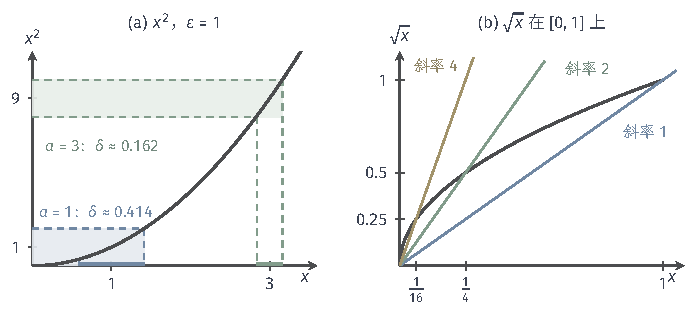
\includegraphics[width=116.695mm]{figures/02-abstract-mathematics/01-metric-and-measure/tikz/c1-uniform-continuity/figure.pdf}
  \caption{连续性中容差随位置的变化。(a) $f(x)=x^2$，取输出容差$\varepsilon=1$：在$a=1$处输入可以偏离$\sqrt2-1\approx0.414$，在$a=3$处只能偏离$\sqrt{10}-3\approx0.162$，曲线越陡，可用的输入区间越窄，在全实轴上没有统一的$\delta$。(b) $f(x)=\sqrt x$在$[0,1]$上：过点$(t,\sqrt t)$与原点的割线斜率$1/\sqrt t$在$t\to0$时无界，图中画出$t=1,\ 1/4,\ 1/16$三条割线，斜率依次为$1,\ 2,\ 4$；不存在统一的Lipschitz常数，但$\sqrt x$在$[0,1]$上仍一致连续。}
  \label{fig:metric-uniform-continuity}
\end{figure*}

\paragraph{一致连续映射保持柯西列}
若$f$一致连续而$(x_n)$是$D$中的柯西列，对$\varepsilon>0$取一致连续的$\delta$，再取$N$使$m,n\geq N$时$d_X(x_m,x_n)<\delta$，则$d_Y(f(x_m),f(x_n))<\varepsilon$，所以$(f(x_n))$是柯西列。逐点连续做不到这一点：$f(x)=1/x$在$(0,1)$上连续，柯西列$1/(n+1)$的像$n+1$却不是柯西列。另一方面，保持柯西列不等于输出有极限：恒等映射$(0,1)\to(0,1)$一致连续，柯西列$1/(n+1)$的像仍是它自己，在陪域$(0,1)$中没有极限。输出极限是否存在取决于陪域是否完备。

\subsection{Lipschitz映射}
\label{sec:metric-lipschitz}

一致连续只保证存在统一的$\delta$，没有说明$\delta$与$\varepsilon$的数量关系。很多误差估计需要更具体的结论：输出误差不超过输入误差的固定倍数。

\begin{definition}[Lipschitz映射]
\label{def:metric-lipschitz}
若存在常数$L\geq0$，使所有$x,y\in D$都满足
\[
  d_Y(f(x),f(y))\leq L\,d_X(x,y),
\]
就称$f$是\term{Lipschitz映射}（Lipschitz map），$L$称为Lipschitz常数。若每个$a\in D$都有半径$r_a>0$与常数$L_a$，使上式在$D\cap B(a,r_a)$上以$L_a$成立，就称$f$\term{局部Lipschitz}（locally Lipschitz）。
\end{definition}

全局Lipschitz推出一致连续：$L>0$时取$\delta=\varepsilon/L$，$L=0$时$f$为常值，任取$\delta$即可。局部Lipschitz推出连续：在$a$处取$\delta=\min\{r_a,\varepsilon/(L_a+1)\}$，则$d_X(x,a)<\delta$时$d_Y(f(x),f(a))\leq L_a\delta<\varepsilon$。局部常数$L_a$可以随$a$无限增大，这时没有全局常数。由反向三角不等式~\eqref{eq:metric-reverse-triangle}，对固定的$z$，$x\mapsto d_X(x,z)$是Lipschitz常数为$1$的映射；同样，由式~\eqref{eq:metric-distance-to-set}定义的$x\mapsto d_X(x,A)$也是$1$-Lipschitz的：对任意$a\in A$，$d_X(x,A)\leq d_X(x,a)\leq d_X(x,y)+d_X(y,a)$，对$a$取下确界得$d_X(x,A)\leq d_X(x,y)+d_X(y,A)$，交换$x,y$即得。

\paragraph{三种条件的区分}
两个例子说明三种条件确实不同。$\sqrt x$在$[0,1]$上一致连续：对$0\leq y\leq x$，$(\sqrt x-\sqrt y)^2\leq(\sqrt x-\sqrt y)(\sqrt x+\sqrt y)=x-y$，所以$|\sqrt x-\sqrt y|\leq\sqrt{|x-y|}$，取$\delta=\varepsilon^2$即可。但它不是Lipschitz映射：$|\sqrt t-\sqrt0|/|t-0|=1/\sqrt t$在$t\to0$时无界，见图~\ref{fig:metric-uniform-continuity}(b)。$x^2$在$\mathbb R$上局部Lipschitz：在$B(a,1)$中$|x^2-y^2|\leq(2|a|+2)|x-y|$；但例~\ref{ex:metric-square-uniform}已经说明它不一致连续，更不是全局Lipschitz。于是在固定定义域和两端度量时，
\[
  \begin{gathered}
    \text{Lipschitz}\Longrightarrow\text{一致连续}\Longrightarrow\text{连续},\\
    \text{Lipschitz}\Longrightarrow\text{局部Lipschitz}\Longrightarrow\text{连续},
  \end{gathered}
\]
各个反向蕴含都不成立。改变定义域或度量后，这些判断需要重新检查。

\subsection{紧致集上的连续映射}
\label{sec:metric-compact-continuous}

第~\ref{sec:metric-compactness}节的紧致性与本节的连续性结合，可以回答两个前面留下的问题：连续函数何时取到最值，下确界$d(x,A)$何时由最近点达到；还能说明紧致定义域上逐点连续何时升级为一致连续。

\begin{theorem}[连续像保持紧致]
\label{thm:metric-compact-image}
若$K$紧致而$f:K\to Y$连续，则$f(K)$是$Y$中的紧致集。特别地，若$K$非空，连续函数$f:K\to\mathbb R$在$K$上取得最大值和最小值。
\end{theorem}

\begin{proof}
设$\{V_\alpha\}$是$Y$中覆盖$f(K)$的一族开集。由定理~\ref{thm:metric-open-preimage}，每个$f^{-1}(V_\alpha)$是$K$中的开集，它们覆盖$K$。由紧致性，有限个$f^{-1}(V_{\alpha_i})$（$i=1,\dots,k$）覆盖$K$，于是$V_{\alpha_1},\dots,V_{\alpha_k}$覆盖$f(K)$。

对实值函数，$f(K)$是$\mathbb R$中的非空紧致集，因而有界且闭。令$s=\sup f(K)<\infty$，由上确界的性质，对每个$n$有$f(K)$中的点大于$s-1/n$，所以$s\in\overline{f(K)}=f(K)$，即存在$x^\star\in K$使$f(x^\star)=s$。最小值同理。
\end{proof}

\paragraph{最近点的存在}
对固定点$x\in X$，映射$a\mapsto d(x,a)$是$1$-Lipschitz的，因而连续。若$A$是非空紧致集，由定理~\ref{thm:metric-compact-image}，它在某个$a^\star\in A$处取到最小值，即$d(x,a^\star)=d(x,A)$：最近点存在。这回答了第~\ref{sec:metric-closure}小节的问题：在$d(2,(0,1))=1$的例子中，$(0,1)$不紧致，下确界没有达到；换成紧致的$[0,1]$，最近点$1$就存在。最近点不一定唯一：原点到单位圆周$S^1$上每一点的距离都是$1$，每一点都是最近点。

\paragraph{连续升级为一致连续}
第~\ref{sec:metric-uniform-continuity}小节中，$x^2$在$\mathbb R$上找不到统一容差，是因为基点可以无限远离原点。紧致定义域排除了这种情形。

\begin{theorem}[紧致集上的一致连续]
\label{thm:metric-compact-uniform}
若$K$紧致而$f:K\to Y$连续，则$f$在$K$上一致连续。
\end{theorem}

\begin{proof}
若不然，存在$\varepsilon>0$，使对每个$\delta=1/n$都有$x_n,y_n\in K$满足$d_X(x_n,y_n)<1/n$而$d_Y(f(x_n),f(y_n))\geq\varepsilon$。由定理~\ref{thm:metric-compact-sequential}，取子列$x_{n_k}\to x\in K$。由$d_X(y_{n_k},x)\leq d_X(y_{n_k},x_{n_k})+d_X(x_{n_k},x)\to0$，也有$y_{n_k}\to x$。由$f$在$x$处连续及序列判据，$f(x_{n_k})\to f(x)$且$f(y_{n_k})\to f(x)$，于是$d_Y(f(x_{n_k}),f(y_{n_k}))\leq d_Y(f(x_{n_k}),f(x))+d_Y(f(x),f(y_{n_k}))\to0$，与它始终不小于$\varepsilon$矛盾。
\end{proof}

这一定理给出统一的容差，但不给出Lipschitz常数：$\sqrt x$在紧致的$[0,1]$上连续，因而一致连续，却不是Lipschitz映射。它也解释了例~\ref{ex:metric-square-uniform}：$[-M,M]$紧致，$x^2$在其上一致连续；$\mathbb R$不紧致，结论不再成立。
